\section{Problem Formalization}\label{statements}
\noindent \sys is an architecture that addresses the correctness and efficiency problems.

\subsection{Statistical Modeling}
In this paper, we will use the term \emph{statistical modeling} to describe a well studied class of analytics problems; ones that can be expressed as the minimization of convex loss functions.
This class is restricted to supervised Machine Learning.
Examples include linear models (including linear and logistic regression), support vector machines, and in fact, means and medians are also special cases. 

Formally, suppose $x$ is a feature vector and $y$ is a label.
For labeled training examples $\{(x_{i},y_{i})\}_{i=1}^{N}$, the problem is to find a vector of \emph{model parameters} $\theta$ by minimizing a loss function $\phi$ (a function that measures prediction error) over all training examples:
\[
 \theta^{*}=\arg\min_{\theta}\sum_{i=1}^{N}\phi(x_{i},y_{i},\theta)
\]
Where $\phi$ is a convex function in $\theta$.
For example, in a linear regression $\phi$ is:
\[
\phi(x_{i},y_{i},\theta) = \|\theta^Tx_{i} - y_i \|_2^2
\]
Sometimes, a \emph{regularization} term $r(\theta)$ is added to the loss, however, this will not affect our results, and we ignore this term without loss of generality.

\subsection{Data Cleaning}
We assume that there is a one-to-one mapping between records in a relation $R$ and labeled training examples $(x_{i},y_{i})$.
%\sys supports two types of data cleaning operations attribute value transformations and removal.
We represent the data cleaning operation as a general user-defined function $C(\cdot)$ that can be applied to a record $r$ and can perform two actions: recover a unique clean record $r' = C(r)$ with the same schema or remove the record $\emptyset = C(r)$.
$C(\cdot)$ can be implemented with software or represent a manual action by the analyst.
We define the clean relation as a relation of all of the records after cleaning:
\[R_{clean} = \cup_i^N C(r_i \in R)\]
Therefore, for every $r' \in R_{clean}$ there exists a unique $r \in R$ in the dirty data.
We acknowledge that this definition is limited as it does \emph{not} cover errors that simultaneously affect multiple records such as record duplication or structure such as schema transformation.
However, the supported cleaning operations include resolving common inconsistencies (e.g., merging ``U.S.A" and ``United States"), filtering outliers (e.g., removing records with values $>1e6$), and standardizing attribute semantics (e.g., ``1.2 miles" and ``1.93 km").
These errors are very common in the context of statistical models for sensor, log, and human-input datasets. 

The record-by-record cleaning model is not a fundamental restriction of \sys, and our technical report discusses a generalization called the ``set of records" cleaning model~\cite{activecleanarxiv}.
In this generalization, the $C(\cdot)$ function is composed of schema preserving \textsf{map} and \textsf{filter} operations applied to the entire dataset.
This can model problems such batch resolution of inconsistencies with a ``find-and-replace".

\subsection{Notation}\label{notation}
The user provides a relation $R$, a cleaner $C(\cdot)$, a featurizer $F(\cdot)$, and a convex loss problem defined by the loss $\phi(\cdot)$.
A total of $k$ records will be cleaned in batches of size $b$, so there will be $\frac{k}{b}$ iterations.  The choice of $b$ does affect the convergence rate.
Section~\ref{model-update} discusses the efficiency and convergence trade-offs of different values of $b$.
We empirically find that a batch size of $50$ performs well across different datasets and use that as a default.
A cleaning budget $k$ can be used as a stopping criterion once $C(\dot)$ has been called $k$ times, and so the number of iterations of \sys is $T = \frac{k}{b}$.
Alternatively, the user can clean data until the model is of sufficient accuracy to make a decision.

We use the following notation to represent relevant intermediate states:

\vspace{0.25em}

\noindent\textbf{Dirty Model: } $\theta^{(d)}$ is the model trained on $R$ (without cleaning) with the featurizer $F(\cdot)$ and loss $\phi(\cdot)$. This serves as an initialization to \sys.

\vspace{0.25em}

\noindent\textbf{Dirty Records: } $R_{dirty} \subseteq R$ is the subset of records that are still dirty. As more data are cleaned $R_{dirty} \rightarrow \{\}$.

\vspace{0.25em}

\noindent\textbf{Clean Records: } $R_{clean} \subseteq R$ is the subset of records that are clean, i.e., the complement of $R_{dirty}$.

\vspace{0.25em}

\noindent\textbf{Samples: } $S$ is a sample (possibly non-uniform but with known probabilities) of the records $R_{dirty}$. The clean sample is denoted by $S_{clean} = C(S)$.

\vspace{0.25em}

\noindent\textbf{Clean Model: } $\theta^{(c)}$ is the optimal clean model, i.e., the model trained on a fully cleaned relation.

\noindent\textbf{Current Model: } $\theta^{(t)}$ is the current best model at iteration $t \in \{1,...,\frac{k}{b}\}$, and $\theta^{(0)} = \theta^{(d)}$. 

\vspace{1.5em}

There are two main metrics that we will use to measure the performance of \sys:

\vspace{0.25em}

\noindent\textbf{Model Error. } The model error is defined as $\|\theta^{(t)} - \theta^{(c)}\|$.

\vspace{0.25em}

\noindent\textbf{Testing Error. } Let $err(\theta^{(t)})$ be the out-of-sample testing error when the current best model is applied to the clean data, and $err(\theta^{(c)})$ be the test error when the clean model is applied to the clean data. The testing error is defined as $err(\theta^{(t)}) - err(\theta^{(c)})$

\subsection{Problem 1. Correctness Problem}\label{updp}
Given newly cleaned a newly cleaned sample $S_{clean}$ and the current best model $\theta^{(t)}$, the model update problem is to calculate $\theta^{(t+1)}$. 
$\theta^{(t+1)}$ will have some error with respect to the true model $\theta^{(c)}$, which we denote as:
\[
error(\theta^{(t+1)}) = \| \theta^{(t+1)} - \theta^{(c)} \|
\]
Since the sample is potentially stochastic, it is only meaningful to talk about expected errors.
We call the update algorithm ``reliable" if the expected error is upper bounded by a monotonically decreasing function $\mu$ of the amount of cleaned data:
\[
\mathbb{E}(error(\theta^{new})) = O(\mu(\mid S_{clean} \mid))
\]
Intuitively, ``reliable" means that more cleaning should imply more accuracy.

\vspace{0.5em}

\emph{The Correct Update Problem is to reliably update the model $\theta^{(t)}$ with a sample of cleaned data.}

\subsection{Problem 2. Efficiency Problem}\label{optp}
The efficiency problem is to select $S_{clean}$ such that the expected error $\mathbb{E}(error(\theta^{(t)}))$ is minimized.
\sys uses previously cleaned data to estimate the value of data cleaning on new records.
Then it draws a sample of records $S \subseteq R_{dirty}$. 
This is a non-uniform sample where each record $r$ has a sampling probability $p(r)$ based on the estimates.
We derive the optimal sampling distribution for the updates, and show how the theoretical optimum can be approximated.

\vspace{0.5em}

\emph{The Efficiency Problem is to select a sampling distribution $p(\cdot)$ over all records such that the expected error w.r.t the model if trained on fully clean data is minimized.}

\subsection{Data Flow and Example}
Figure \ref{sys-arch} illustrates the \sys architecture.
The system first trains the model $\phi(\cdot)$ on the dirty dataset to find an initial model $\theta^{(d)}$ that the system will subsequently improve.
The {\it sampler} selects a sample of size $b$ records from the dataset and passes
the sample to the {\it cleaner}, which executes $C(\cdot)$ for each sample record and outputs their cleaned versions.
The \emph{updater} uses the cleaned sample to update the weights of the model, thus moving the model closer to the true cleaned model (in expectation).
Finally, the system either terminates due to a stopping condition (e.g., $C(\cdot)$ has been called a maximum number of times $k$, or training error convergence),
or passes control to the {\it sampler} for the next iteration.

A user provided {\it Detector} can be used to identify such records that are more likely to be dirty, and thus improves the likelihood that the next sample will contain true dirty records.
Furthermore, the {\it Estimator} uses previously cleaned data to estimate the effect that cleaning a given record will have on the model.
These components can be used separately (if only one is supplied) or together to focus the system's cleaning efforts on records that will most improve the model.
Section \ref{opti} describes several instantiations of these components for different data cleaning problems.
Our experiments show that these optimizations can improve model accuracy by up-to 2.5x (Section \ref{comp}).

\begin{figure}[t]
\centering
 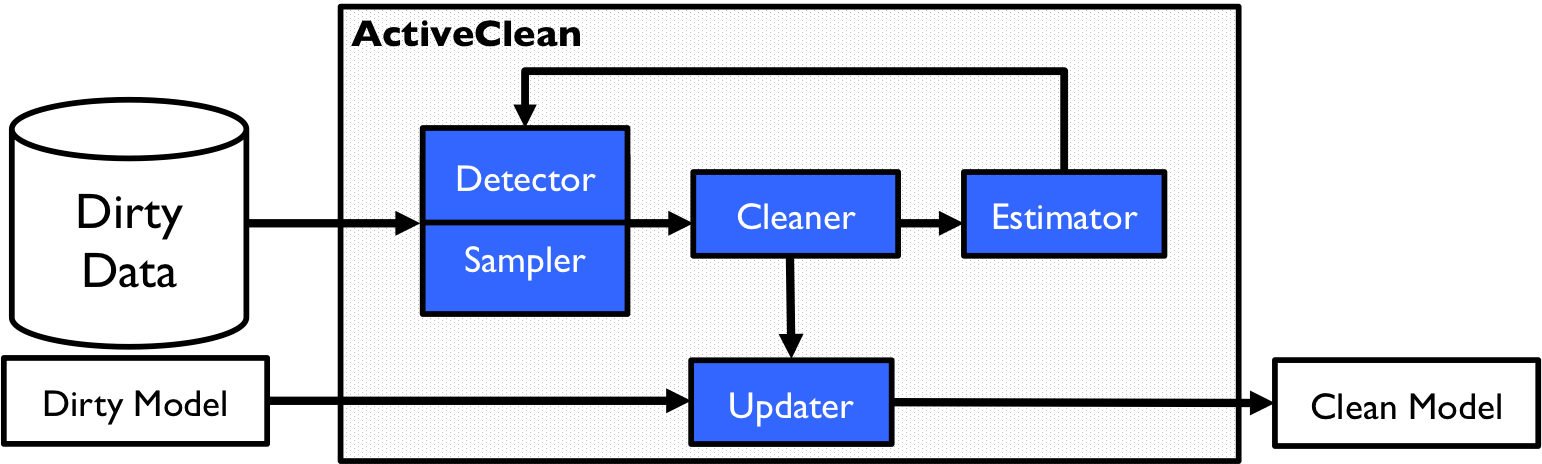
\includegraphics[width=\columnwidth]{figs/arch.png}
 \caption{\sysfull allows users to train predictive models while progressively cleaning data but preserves convergence guarantees. \label{sys-arch}}
\end{figure}


Going back to the ProPublica example in Section~\ref{s:usecase}, we illustrate how \sys can be used:
\begin{example}\label{archex}
The analyst chooses to use an SVM model, and manually cleans records by hand (the $C(\cdot)$).  
\sys initially selects a sample of $50$ records (the default)  to show the analyst.
She identifies a subset of 15 records that are dirty, fixes them by normalizing the drug and corporation names with the help of a search engine, and corrects the labels with typographical or incorrect values.
The system then uses the cleaned records to update the current best model and selects the next sample of $50$.
The analyst can stop at any time and use the improved model to predict donation likelihoods.
\end{example}

\iffalse
\subsection{\sys Problem}
The core problem addressed by \sys is incremental model update while progressively cleaning data.

\begin{problem}[ActiveClean Problem]\label{activeclean}\sloppy
Let $R$ be a dirty relation, $F(r) \mapsto (x,y)$ be a featurization that maps
a record $r \in R$ to a feature vector $x$ and label $y$, $\phi$ be a convex regularized loss,
and $C(r) \mapsto r_{clean}$ be a cleaning technique that maps a record to its cleaned value. 
Given these inputs, the \sys problem is to return a \textbf{reliable} estimate $\hat{\theta}$ of the clean model for any limit $k$ on the number of times the data cleaning $C(\cdot)$ can be applied.

\vspace{0.5em}

\textbf{Reliable} precisely means that the expected error in this estimate (i.e., L2 difference w.r.t a model trained on a fully cleaned dataset) is bounded above by a monotonic function in $k$ and a monotonic function of the error in the dirty model.
\end{problem}
\fi


\iffalse
From a systems perspective, data cleaning and model training happen at very different time scales.
When humans are involved, per record latencies for data cleaning are orders of magnitude larger than the CPU time needed for model training.
We can compare recent results in data cleaning to a model training framework like CoCoA implemented on Spark \cite{jaggi2014communication}.
Per record, BigDansing, a highly optimized automated Spark-based data cleaning system is 15.5x slower than CoCoA\footnote{For CoCoA to reach a precision of 1e-3}.
Crowd based techniques like CrowdFill \cite{park2014crowdfill} and CrowdER \cite{wang2012crowder} are over 100,000x slower per record. 
Consequently, all of the optimizations in \sys are designed to address data cleaning latency (i.e., more progress with fewer cleaned records) rather than optimizing for numerical computation (i.e., process fewer records).
\fi



\iffalse
Here is an example application of \sys with our running example:
\begin{example}
The analyst first trains her SVM model on the dirty data ignoring the effects of the errors returning a model $\theta^{(d)}$.
She decides that she has a budget of cleaning $100$ records, and decides to clean the 100 records in batches of 10 (set based on how fast she can clean the data, and how often she wants to see an updated result).
She initializes \sys with $\theta^{(d)}$.
\sys samples an initial batch of 10 records.
She manually cleans those records by merging similar drug names, making corporation names consistent, and fixing incorrect labels.
After each batch, the model is updated with the most recent cleaning results $\theta^{(t)}$.
The model improves after each iteration.
After $t=10$ of cleaning, the analyst has an accurate model trained with 100 cleaned records but still utilizes the entire dirty data.
\end{example}



\subsection{Two perspectives on error}
When faced with such errors there are two contrasting perspectives from the Machine Learning and the Database communities.

\vspace{0.5em}

\noindent\textbf{Existing Database Literature. } 
Traditionally, cleaning is agnostic to the queries and analysis that happens downstream. 
This perspective breaks down when cleaning is so expensive that we can only clean a small number of records.
Ideally, we should clean the records that are most valuable to the downstream analysis.

\vspace{0.5em}

\noindent\textbf{Existing  Machine Learning Literature. } The Machine Learning community has focused on
designing models that are robust to outliers (i.e., values far away from the typical value)
For example, in the case of linear regression, we can change the $L_2$ norm to an $L_1$ norm to mitigate the effect of outliers:
\[
\phi(x_{i}^T\theta,y_{i}) = \|\theta^Tx_{i} - y_i \|_1
\]
The quadratic L2 loss implies that examples that deviate far from the typical example are quadratically penalized as opposed to linearly penalized with the L1 loss.
There is a natural tradeoff between robustness and efficiency.
The more robust a technique is, the less efficient it will be (i.e., estimate variance for a fixed number of training examples).
Robust techniques are best suited for random errors that look significantly different the rest of the examples.
When errors are systematic, the Machine Learning answer has been to design features in such a way that they are robust to some systematic bias.
For example, in image processing, scale-invariant feature transforms (SIFT) are widely applied that allow for image models invariant to pose or scaling issues.

\vspace{0.5em}

\noindent\textbf{The \sys Contribution. } We try to bring two perspectives together in this work to address the problem of expensive to clean systematic errors, namely the Database idea of data cleaning and the Machine Learning formalization of empirical risk minimization.
Some errors require expensive cleaning procedures, increasingly using the crowd, and we joint have a time budget on cleaning and analysis.
\sys prioritizes cleaning with respect to an estimated impact on the clean model.

\subsection{SampleClean Project}

Traditionally, data cleaning has explored expensive, up-front cleaning of entire datasets for increased query accuracy.
We proposed the SampleClean problem, in which an analyst cleans a small sample of data, and then estimates the result to an aggregate query e.g., \sumfunc, \countfunc, or \avgfunc.
The main insight from the SampleClean project is that highly accurate answers for aggregate queries does not require cleaning the full dataset.
Generalizing this insight, there is a deep relationship between the application (i.e., the query) and how an analyst should budget their effort in data cleaning.
In fact, \avgfunc and \sumfunc queries are a special case of the convex loss minimization discussed in the previous section:
\[
\phi = (x_{i} - \theta)^2
\]

We then extended the SampleClean work to study cleaning Materialized Views \cite{technicalReport}.
Suppose base data is updated with insertions, deletions, or updates, we explored how we could efficiently propagate
changes to a sample of the view instead of the full view.
Subsequent queries on the view could be answered approximate.

The SampleClean problem inspired an eponymous system that implements sampling, data cleaning, and approximate query processing on the Apache Spark stack \cite{sampleclean}.
Also included in the Apache Spark stack are Machine Learning libraries including MLlib \cite{mllib} and GraphX \cite{graphx}.
The in-memory architecture of the Apache Spark stack allows for increasingly interactive analysis \cite{AgarwalMPMMS13, armbrust2015spark}.
Analysts can prototype data processing workflows on samples to evaluate performance before running expensive batch processing jobs on entire datasets.
With data cleaning and machine learning libraries in the same software ecosystem, we see a new opportunity for joint optimization for interactive model building.



\subsection{Stochastic Gradient Descent}
Sampling is a natural part of any Machine Learning workflow, as stochastic optimization is widely used to fit model parameters.
The problems described in the previous subsections are often trained using a technique called Stochastic Gradient Descent (SGD) or one of its variants.
The basic idea of SGD is to draw a data point at random, calculate the gradient at that point, and then update a current best estimate with that gradient.
\[
\theta^{(t+1)}\leftarrow\theta^{(t)}-\gamma\nabla\phi(x_{i}^T\theta,y_{i})
\]
 SGD can also be applied in a ``mini-batch" mode, where we draw a subset of data $S^{(t)}$ at random and update with the average gradient.
 \[
 \theta^{(t+1)}\leftarrow\theta^{(t)}-\frac{\gamma}{\|S^{(t)}\|}\sum_{i\in S^{(t)}}\nabla\phi(x_{i}^T\theta,y_{i})
 \]

We can use this workflow for designing an anytime data cleaning methodology.
As data is sampled, we can clean the samples.
The analyst then can stop at anytime and use the best model at that instant.
SGD and its variants are well-studied and there are lower-bounds on the convergence rates using these techniques. 
Recently, a number of works have explored non-uniform sampling distributions for stochastic optimization \cite{zhao2014stochastic, qu2014randomized}.
The main insight is that non-uniform distributions may on average estimate the gradient accurately.
In this work, we explore how to design such a non-uniform distribution for iterative data cleaning.

\fi


 
